\chapter{PUF results and demonstration}
\label{ch:result}

To fully characterise the \acrshort{puf} performance of the two implementations, the following aspects are studied:

\begin{itemize}
    \item The oscillations of the \acrshort{tero} cells over time.
    \item The intra-device metrics (uniformity and reliability) for different acquisition times on a single device.
    \item The inter-device metrics (average uniformity and reliability, uniqueness and bit-aliasing) are computed from the result of 33 devices for a chosen acquisition time.
    \item The impact of the \acrfull{ecc}.
\end{itemize}

Furthermore, the performance found will be compared to other existing \acrshort{teropuf} implementations, followed by a description of the demonstration.\\

All tests are run on Basys-3 with the main clock frequency being 100 MHz. Each data point is averaged over 10 000 samples. The tests were done with an ambient temperature around 20\textdegree C and nominal voltage.\\

The interface between the FPGA and the computer is done via UART and a custom Python module described in appendix~\ref{appendix:python_mod}

\section{Cells behaviour and equalities}

The value of the counter of each cell is directly sent via \acrshort{uart} once the acquisition time is reached, instead of being compared to generate the \acrshort{puf} response. The range of acquisition time to evaluate is chosen from $0.01\mu s$ to $2\mu s$. The expected behaviour is to initially have several oscillations at the beginning, then at some point, reach stability and remain constant.

\subsection{Oscillations over time}
\subsubsection*{TERO-4}

The 64 TERO-4 cell's oscillations are displayed in figure~\ref{fig:tero_4_oscillation_vs_time}. The cells stabilise within a single clock cycle ($0.01\mu s$) with a final number of oscillations below 20, except for one cell that only stabilises around $0.4\mu s$ after 160 oscillations.

\begin{figure}[H]
   \begin{minipage}[b]{\linewidth} 
        \centering
        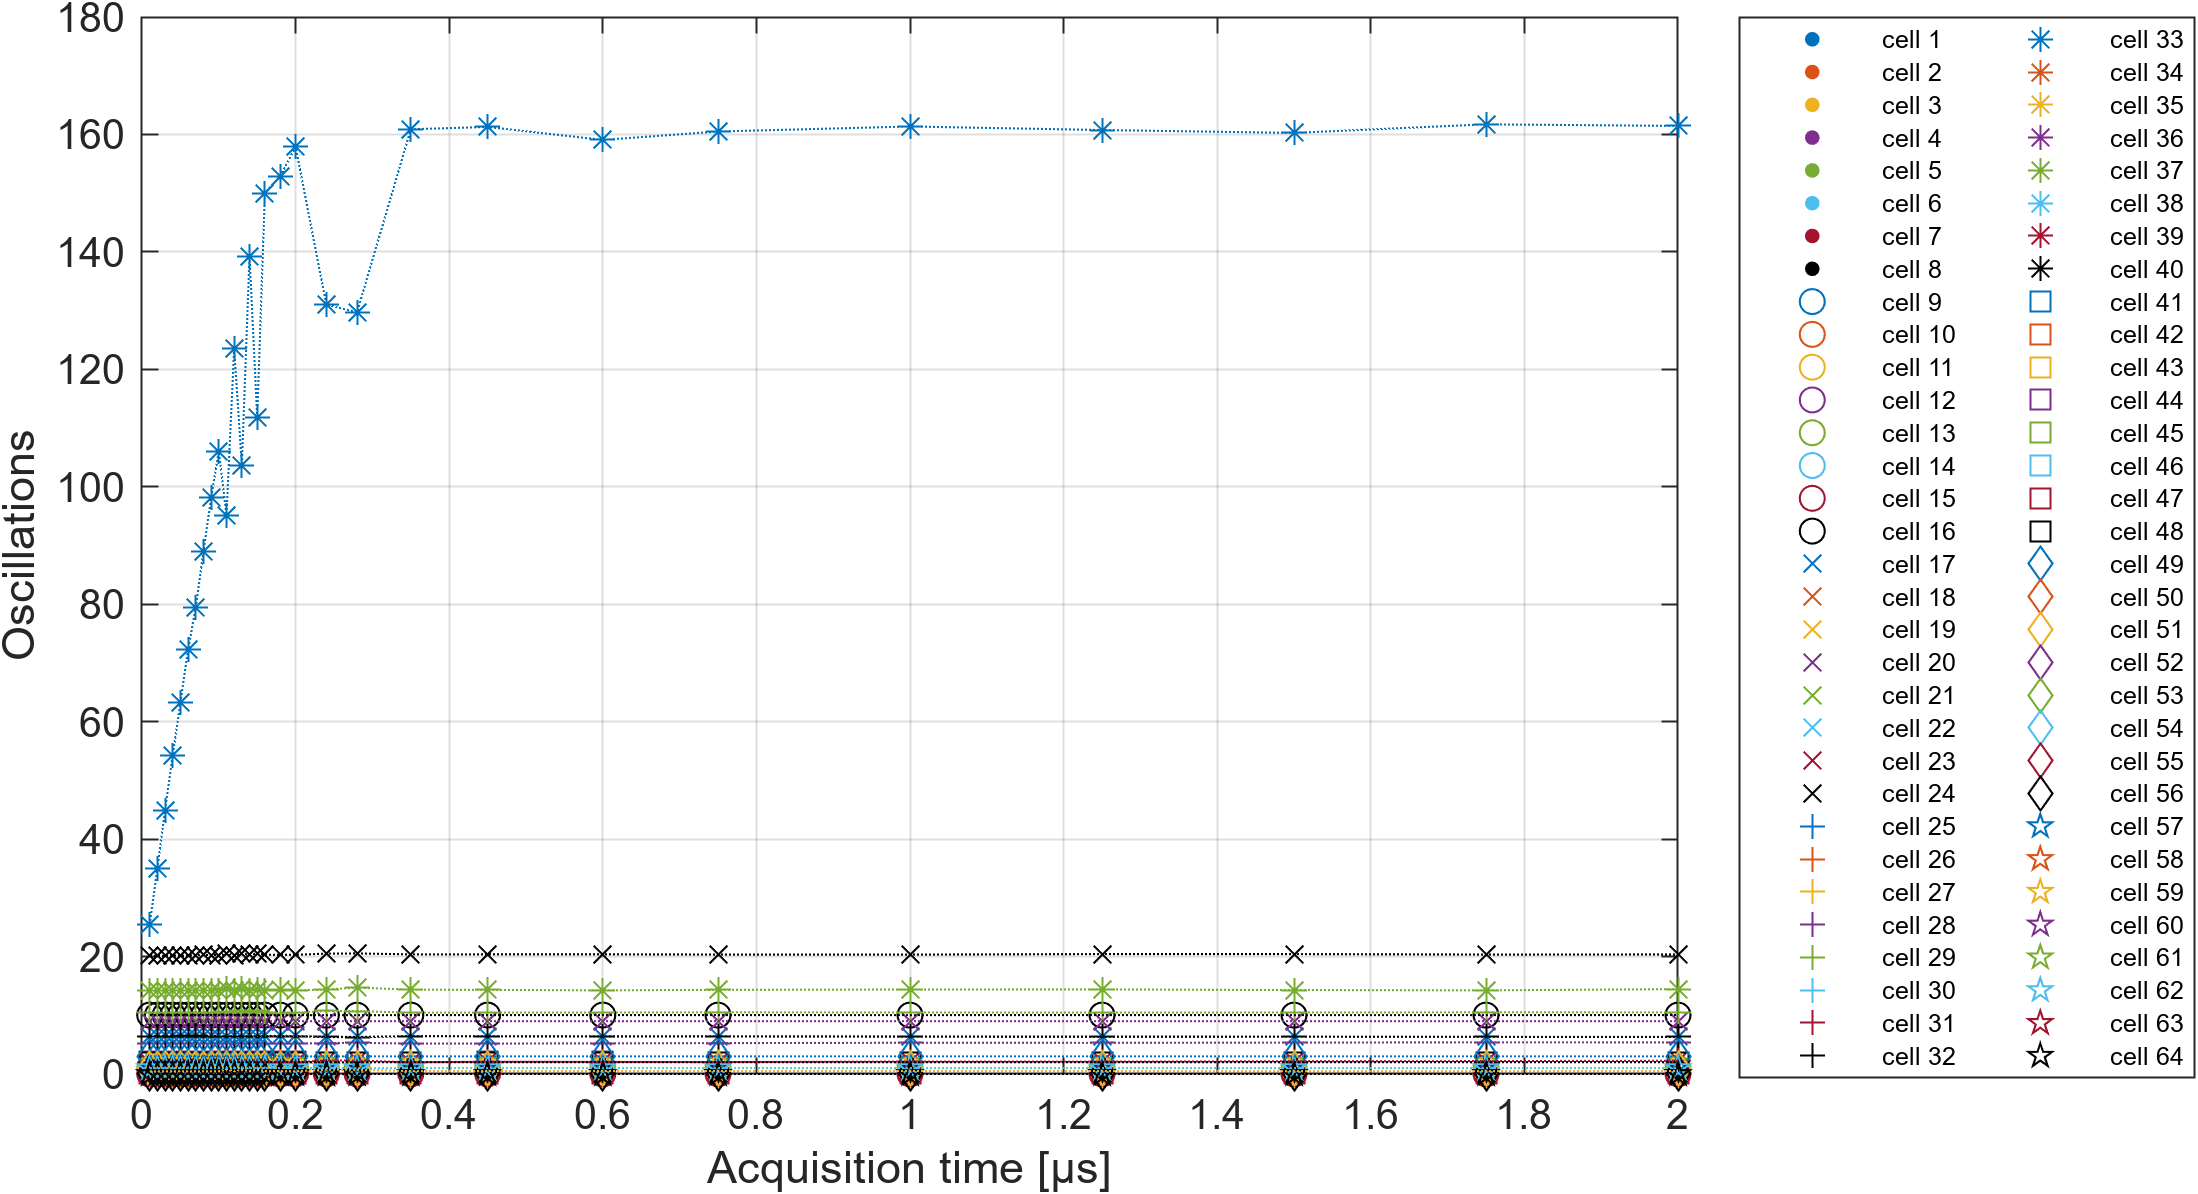
\includegraphics[width=\linewidth]{images/tero_4_oscillations_vs_time.png}
        \subcaption{Full\label{fig:tero_4_oscillation_vs_time_full}}
   \end{minipage}
   \begin{minipage}[b]{\linewidth}   
        \centering
        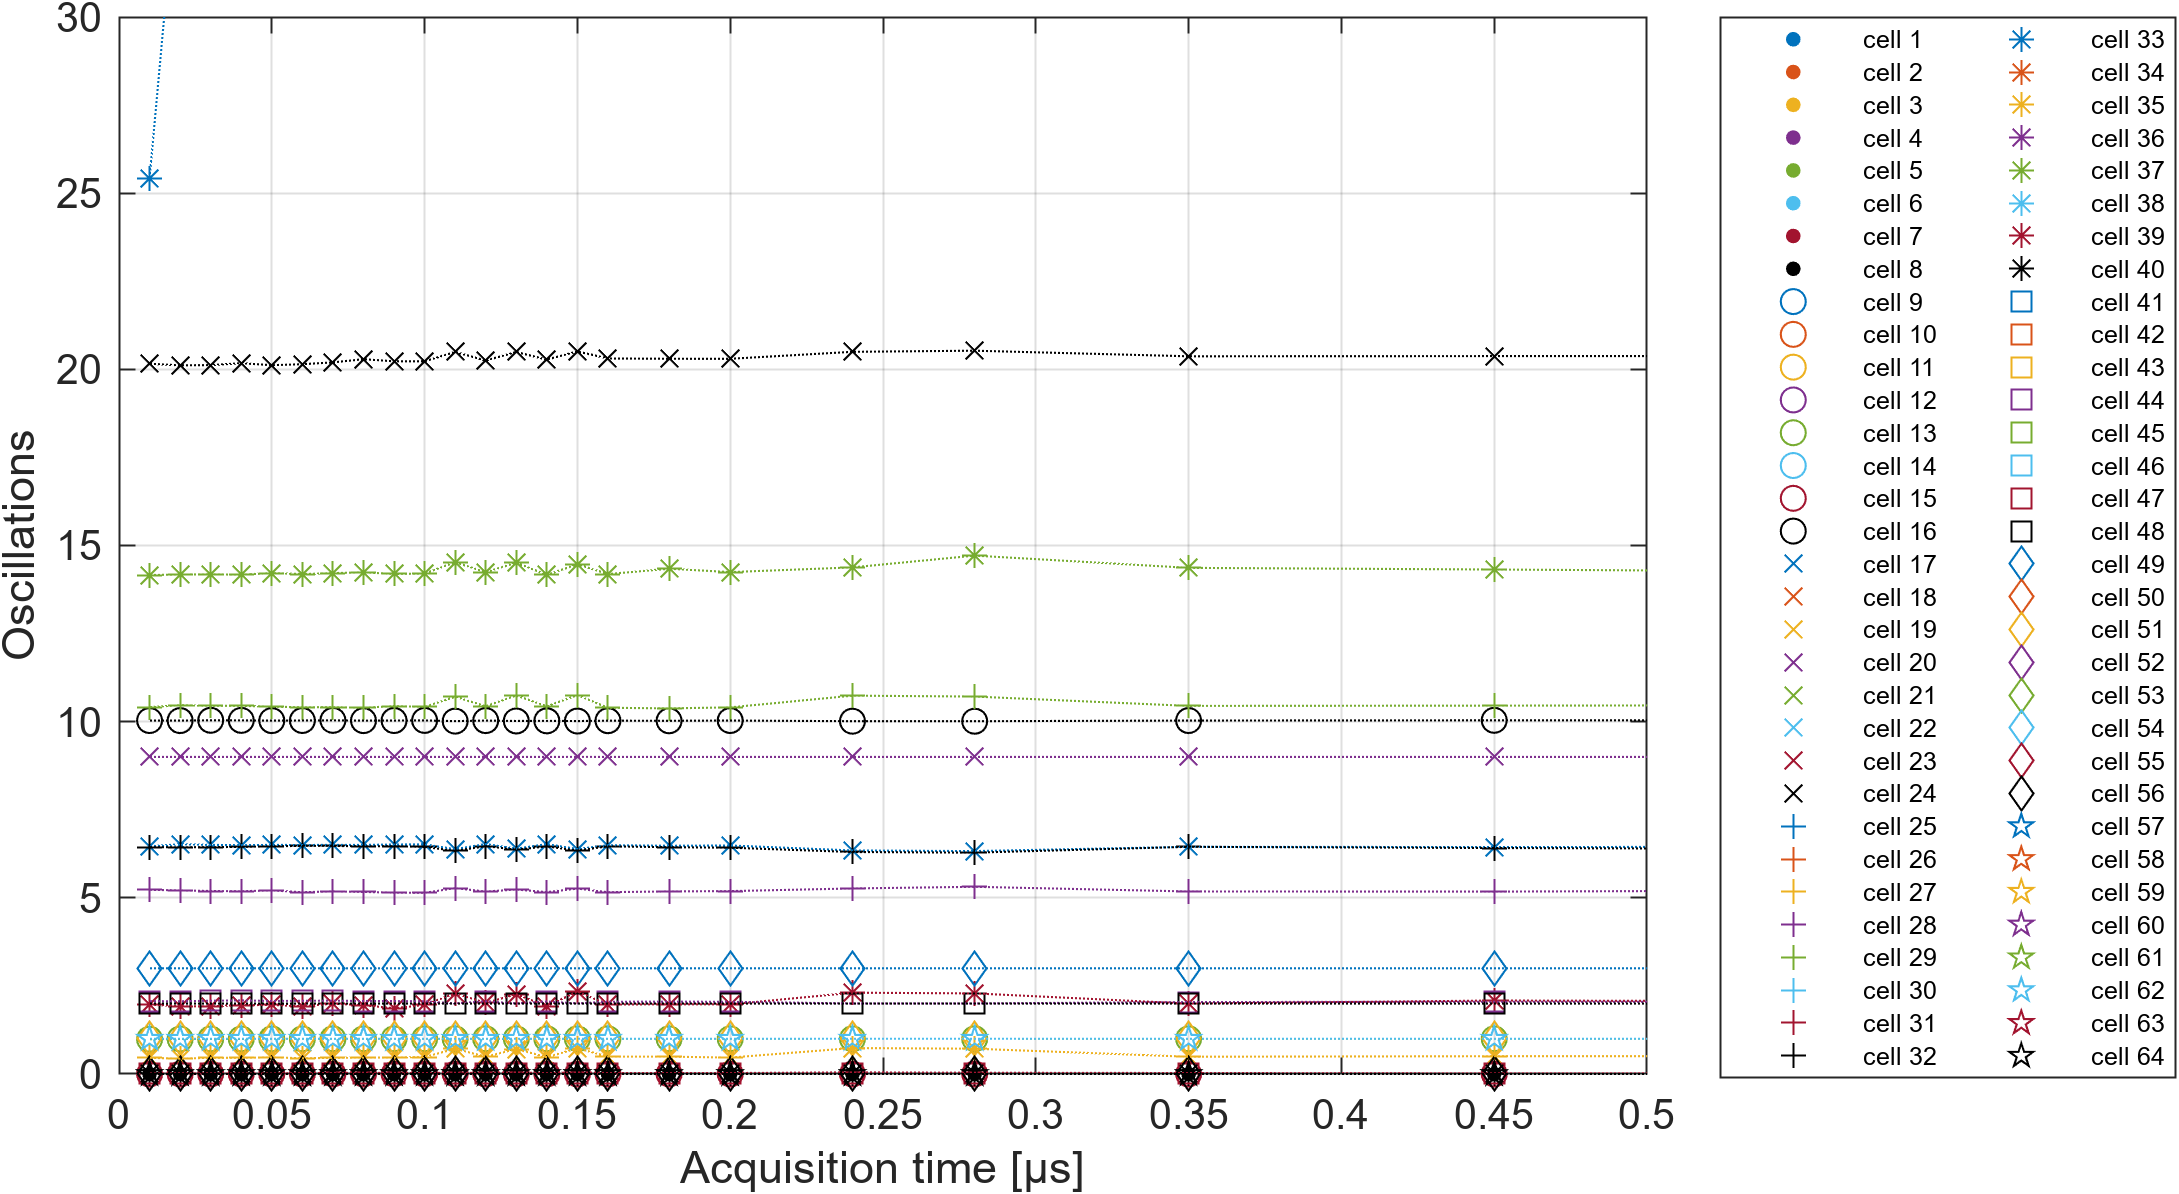
\includegraphics[width=\linewidth]{images/tero_4_oscillations_vs_time_zoomed.png}
        \subcaption{Zoomed\label{fig:tero_4_oscillation_vs_time_zoomed}}
   \end{minipage}
   \caption{TERO-4 cells oscillations over acquisition time\label{fig:tero_4_oscillation_vs_time}}
\end{figure}

\subsubsection*{TERO-8}

The figure~\ref{fig:tero_8_oscillation_vs_time} represents the oscillation of the 64 TERO-8 cells. The stabilisation time is mostly below $0.5 \mu s$. Four cells seem to never really stabilise before $2\mu s$. The final number of oscillations of the stable cells is spread up to 200.\\

\begin{figure}[H]
   \begin{minipage}[b]{\linewidth} 
        \centering
        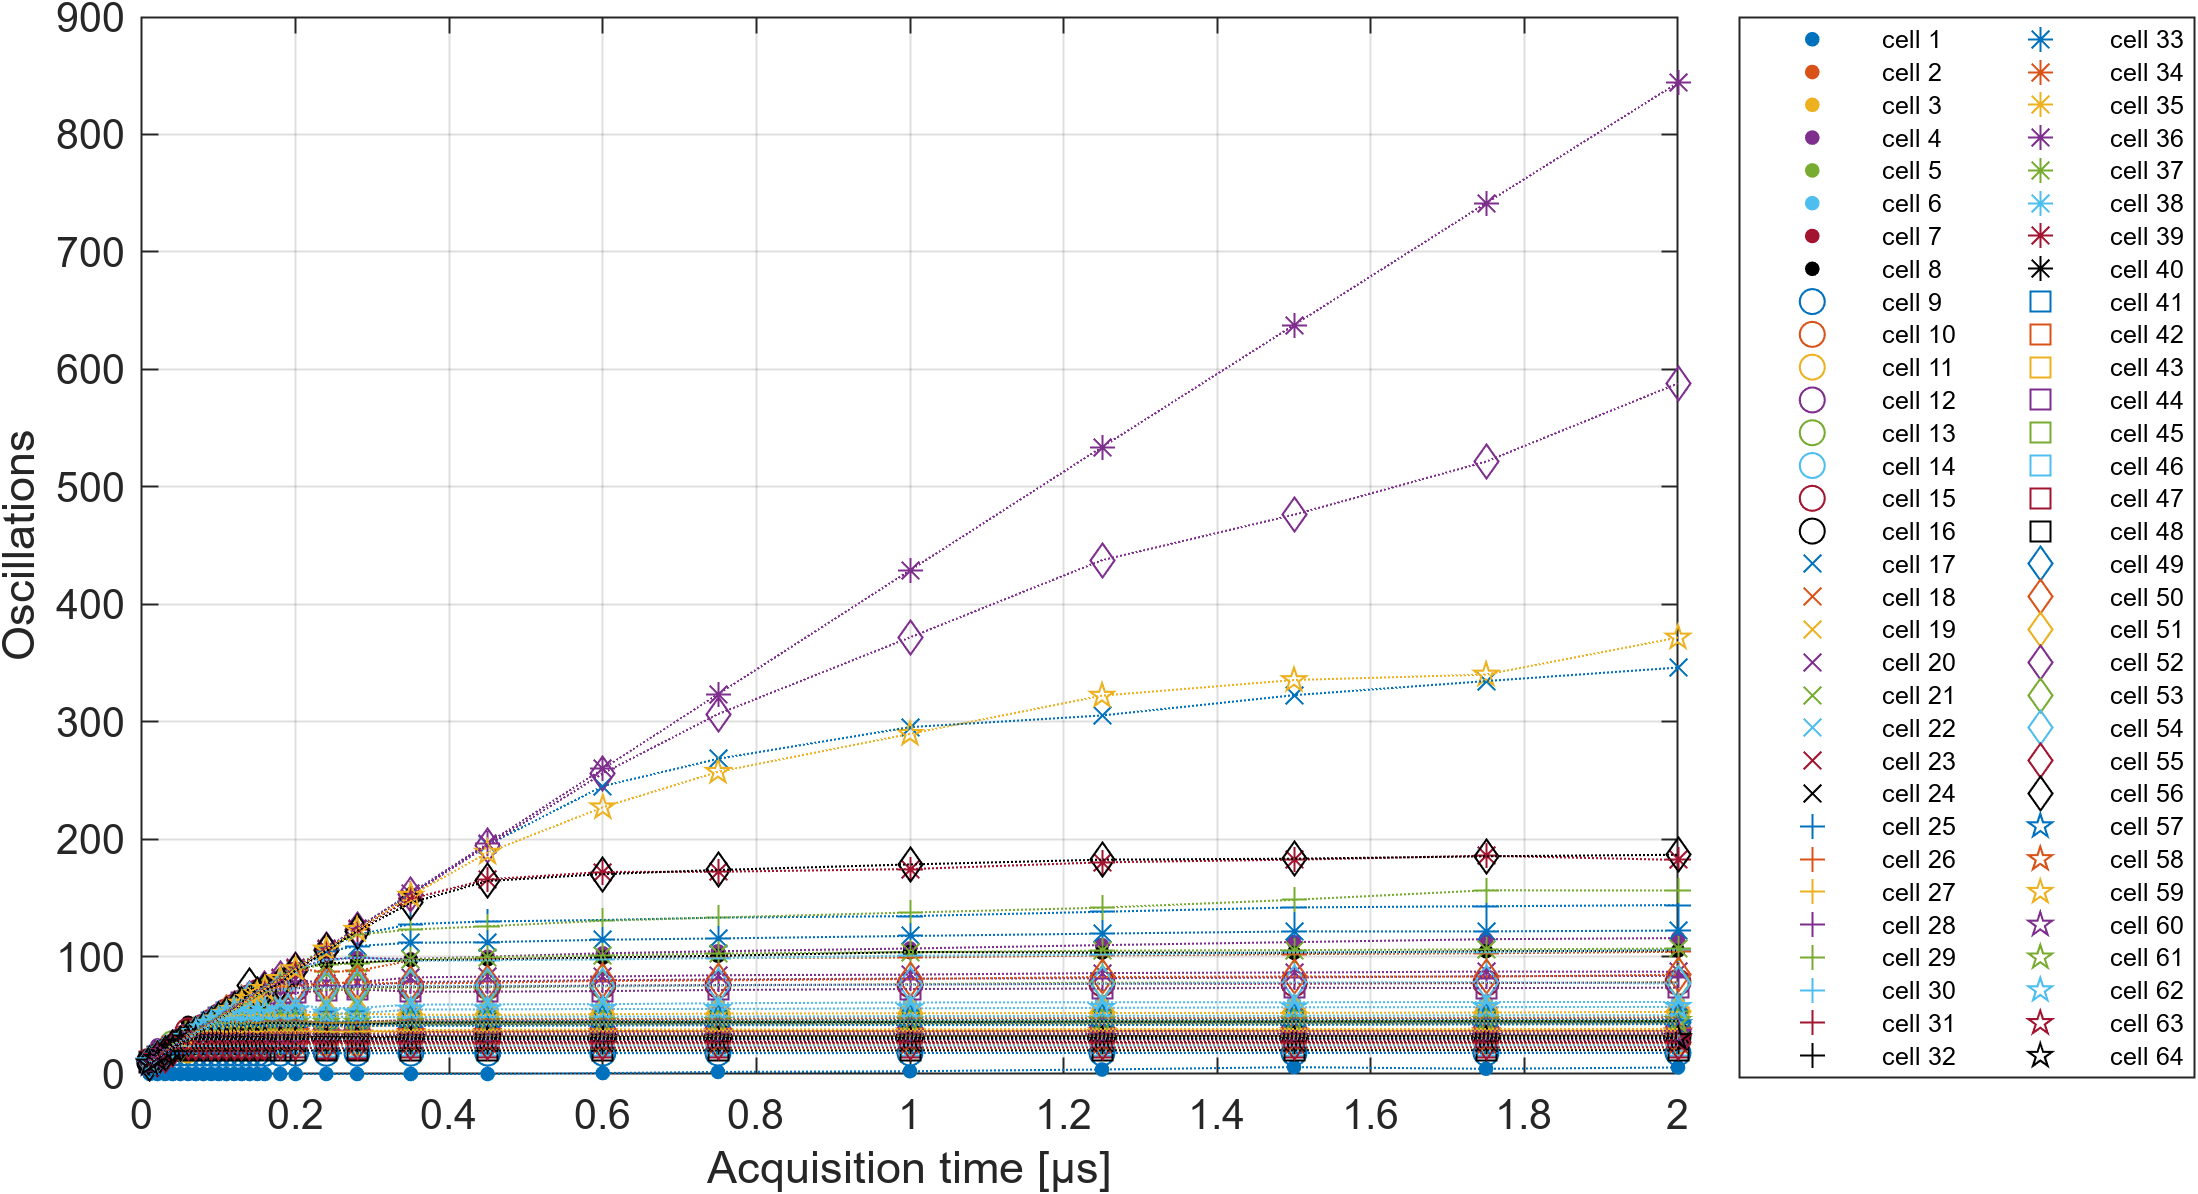
\includegraphics[width=\linewidth]{images/tero_8_oscillations_vs_time.png}
        \subcaption{Full\label{fig:tero_8_oscillation_vs_time_full}}
   \end{minipage}
   \begin{minipage}[b]{\linewidth}   
        \centering
        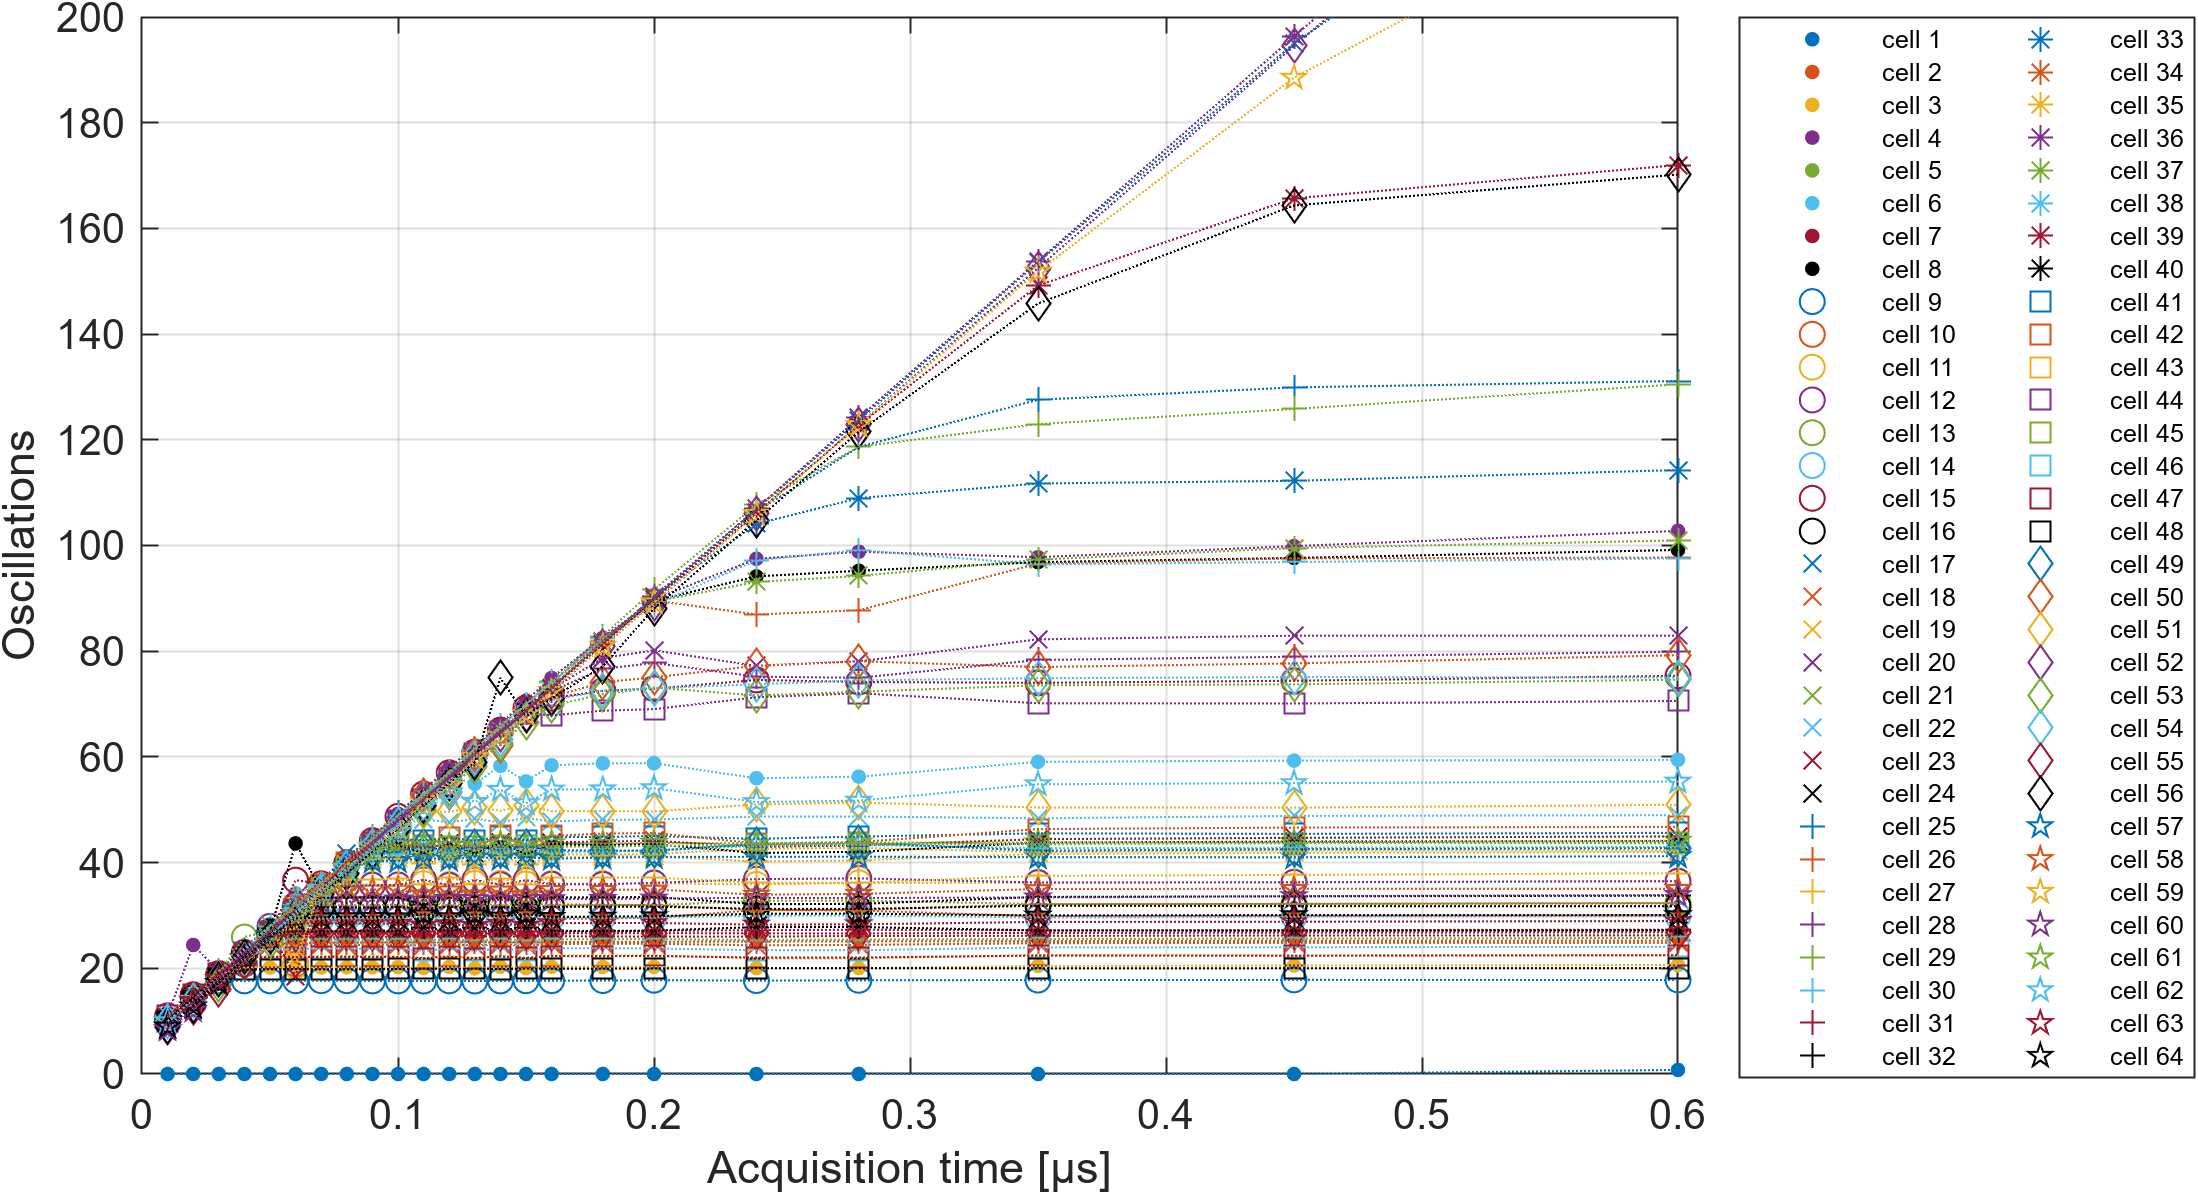
\includegraphics[width=\linewidth]{images/tero_8_oscillations_vs_time_zoomed.png}
        \subcaption{Zoomed\label{fig:tero_8_oscillation_vs_time_zoomed}}
   \end{minipage}
   \caption{TERO-8 cells oscillations over acquisition time\label{fig:tero_8_oscillation_vs_time}}
\end{figure}


Figures \ref{fig:tero_8_oscillation_vs_time_full} and \ref{fig:tero_8_oscillation_vs_time_zoomed} confirm that most of the cells do stabilise and only a few are unstable as expected. If the unstable cells become an issue for the implementation, we could imagine changing the physical location of the unstable cells on the \acrshort{fpga} until all cells are stable. However, this would require a calibration step and this will not be studied in this thesis.


\subsection{Final state}

The final state of the cells (i.e. the number of oscillations after stabilisation) is difficult to see on the previous graphs. Here we display the final state of each cell at $2\mu s$ as a histogram on figures~\ref{fig:tero_both_oscillation_final}. The cells that are considered unstable from the previous section are excluded for more visibility.\\

For the TERO-4, this reveals that 48 of the 64 cells have a final number of oscillations equal to zero, meaning that they do not oscillate a single time. For the TERO-8, the final number of oscillations is more spread than for the TERO-4, with at most 3 cells with the same number.

\begin{figure}[H]
   \begin{minipage}[b]{0.5\linewidth} 
        \centering
        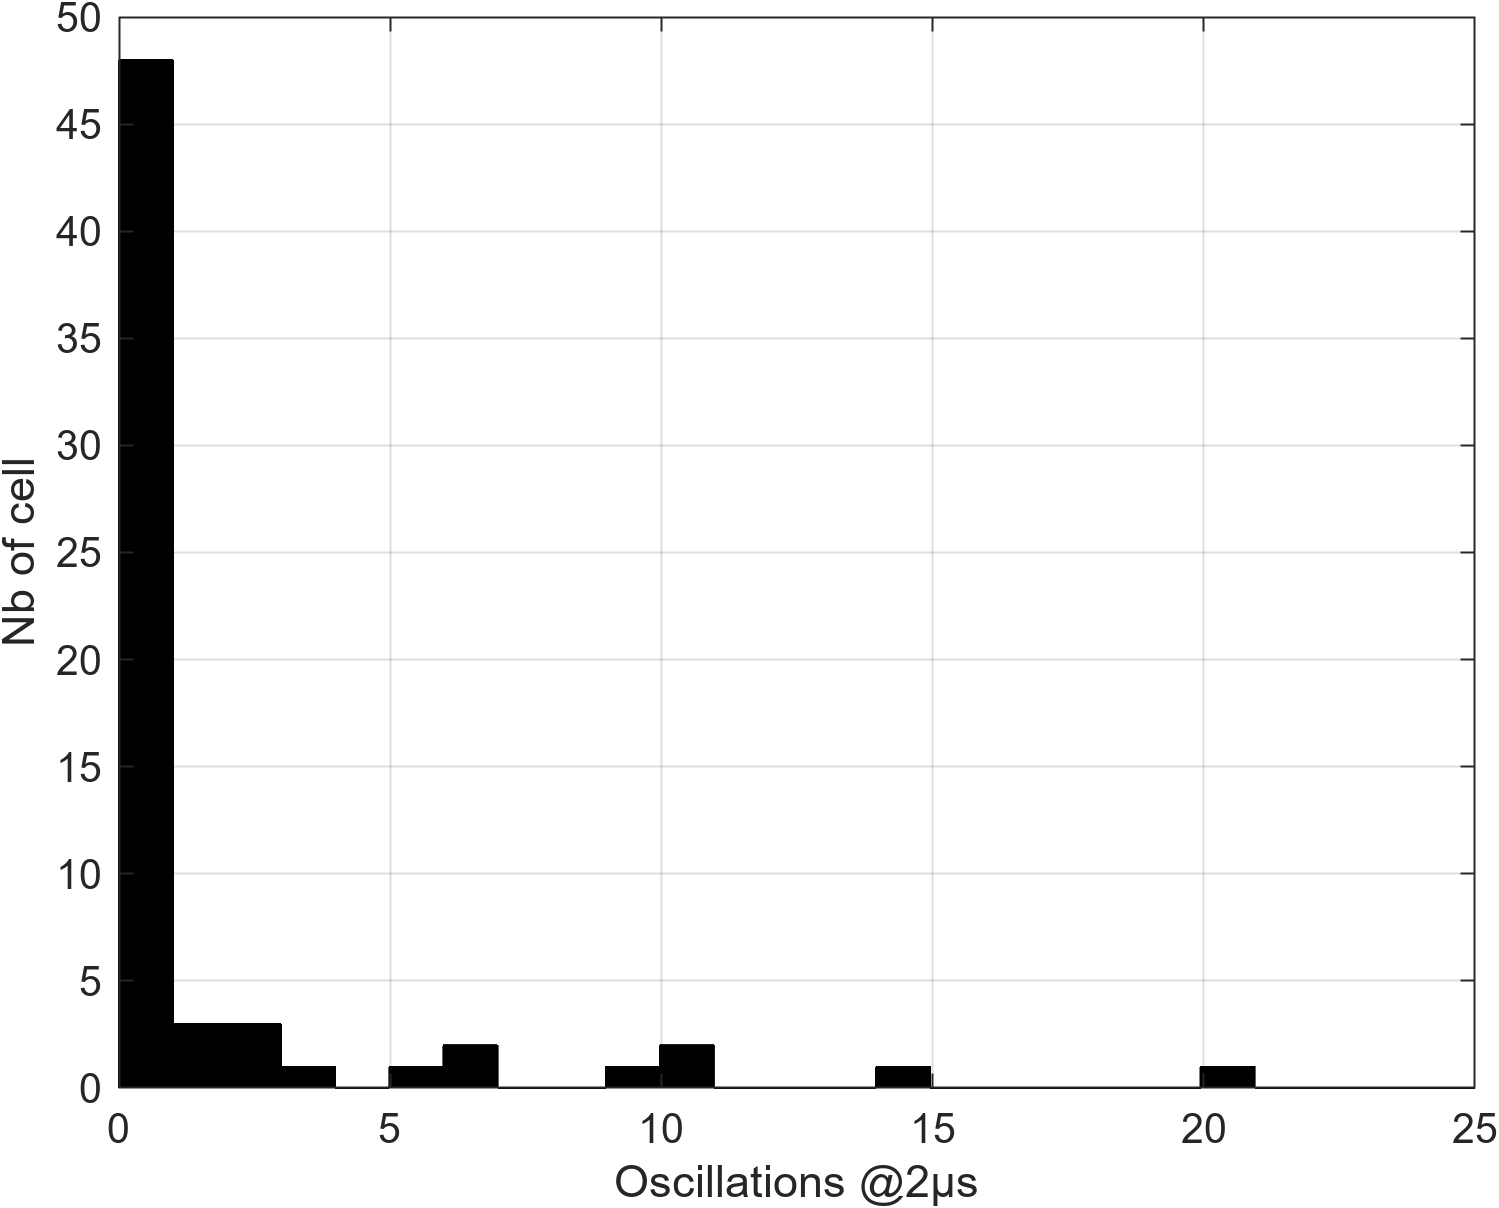
\includegraphics[width=\linewidth]{images/tero_4_oscillations_final.png}
        \subcaption{TERO-4\label{fig:tero_4_oscillation_final}}
   \end{minipage}
   \begin{minipage}[b]{0.5\linewidth}   
        \centering
        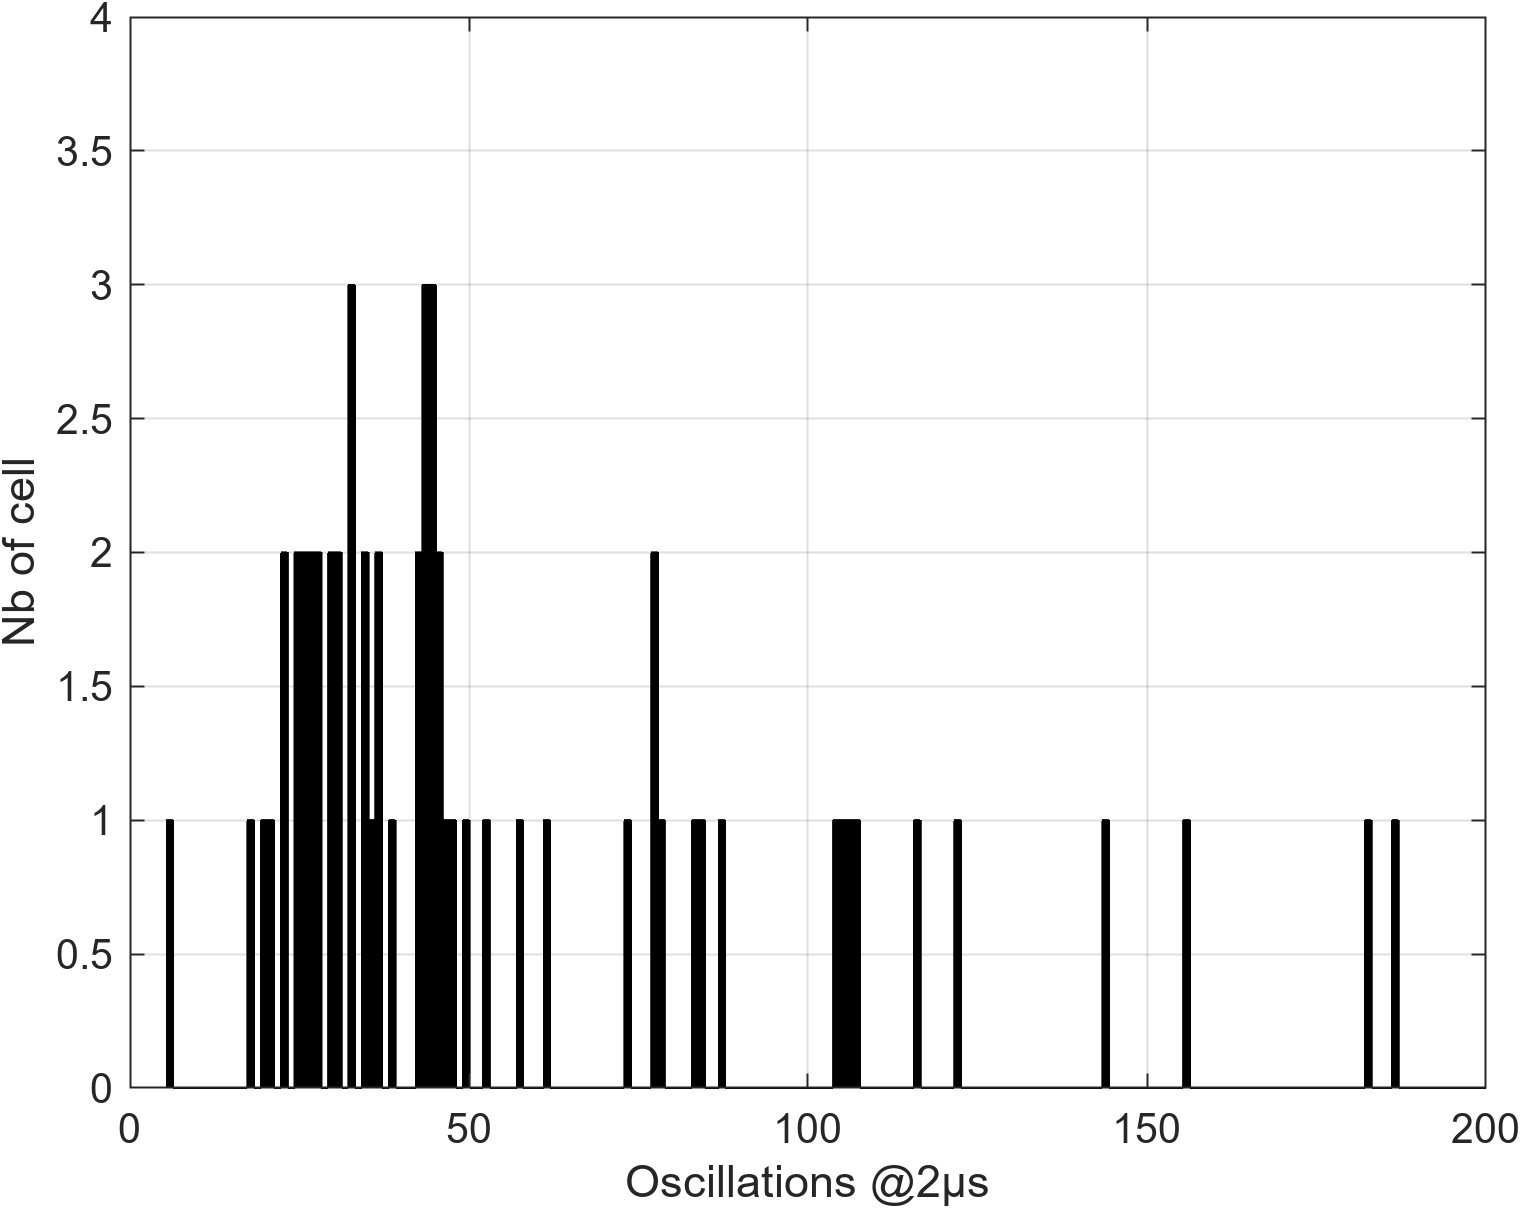
\includegraphics[width=\linewidth]{images/tero_8_oscillations_final.png}
        \subcaption{TERO-8\label{fig:tero_8_oscillation_final}}
   \end{minipage}
   \caption{\acrshort{tero} cells - number of oscillations at $2\mu s$\label{fig:tero_both_oscillation_final}}
\end{figure}




\newpage
\subsection{Equality's}

In the \acrshort{puf} implementation, the bits responses are generated by comparing the number of oscillations of two cells. Therefore, a high proportion of the cell having the same number of oscillations will lead to a high number of equalities in the process. As discussed in the section~\ref{sec:design_generation}, the equality results in a response that is always the same and therefore needs to be avoided as much as possible.


\begin{figure}[H]
    \centering
    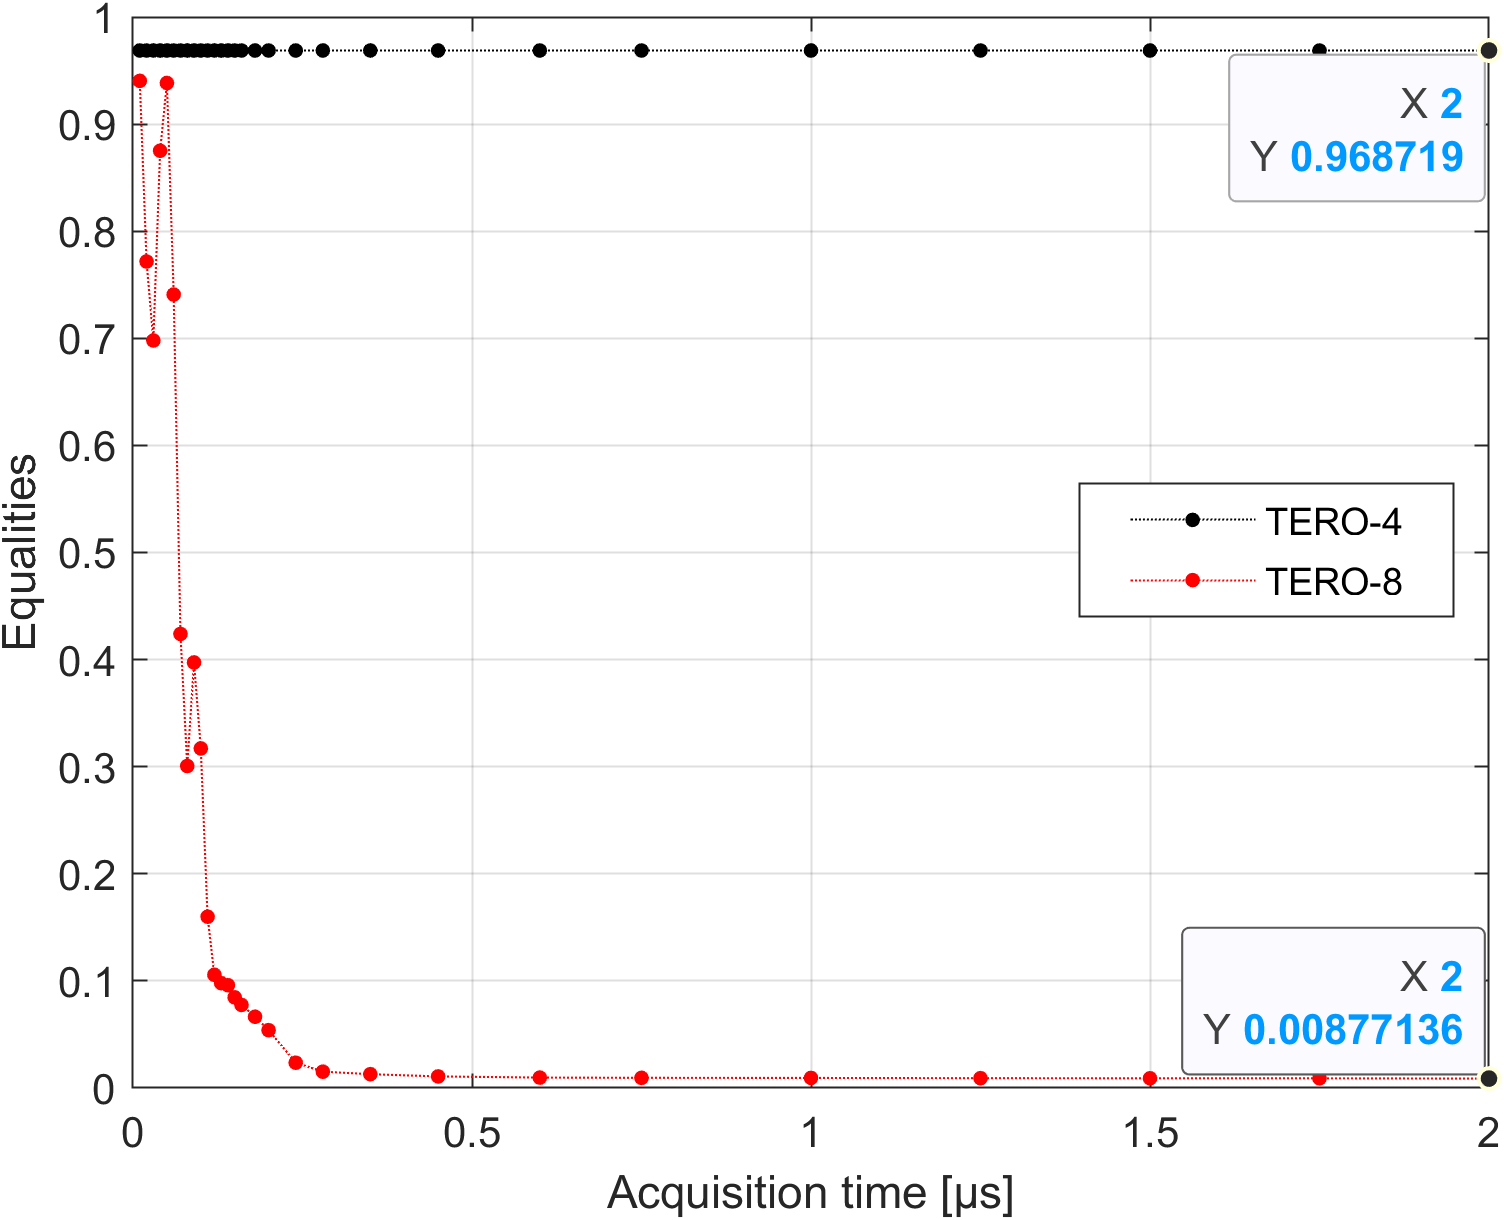
\includegraphics[width=0.8\linewidth]{images/all_oscillations_equality.png}
    \caption{\label{fig:tero_all_oscillation_eq}\acrshort{tero} cells oscillations equality's over acquisition time}
\end{figure}

Comparing each pair of cells similarly than for the response generation, we can find the proportion of equalities, which is shown in figure~\ref{fig:tero_all_oscillation_eq}. The TERO-4 cells comparison raises an equality for 96.8\% of the cells combination, for any acquisition time. The TERO-8 cells however produced less than 1\% of equality after $0.4 \mu s$ and almost 0\% at $2\mu s$. It is also interesting to observe the beginning where there is a high number of equality which decreases rapidly. This is coherent since this is the moment where the cells start to stabilise, each one at a time, and therefore the number of oscillations diverges for each cell.\\

From this test, TERO-4 cells seem to not be suitable due to a high proportion of the cells that do not oscillate, while the TERO-8 cells behave as expected. However, it is possible that another device would produce a completely different behaviour and it could simply be due to unfortunate circumstances.\\


\section{Intra-device performances and acquisition time determination}

This tests studies the intra-device metrics (\acrlong{unif} and \acrlong{relia})  of the \acrshort{puf} for different acquisition times (still between $0.01\mu s$ to $2\mu s$). This provides a first look at the \acrshort{puf} performances on a single device, before the final characterisation with the inter-device metrics. The goal is also to choose an adequate acquisition time to have the best \acrshort{puf} properties for the final test.\\

\subsection{Uniformity}

As defined in the chapter~\ref{ch:1-puf}, \acrfull{unif} is the measure of the response's bit repartition between '0' and '1' and is ideally equal to 50\%. This metric is displayed in figure~\ref{fig:all_intra_uniformity} for both TERO-4 and TERO-8. The uniformity of the TERO-4 PUF stays steady at 3\% while the TERO-8 oscillates shortly then rises and stabilises to 53.0\% around $0.3\mu s$.\\


\begin{figure}[H]
    \centering
    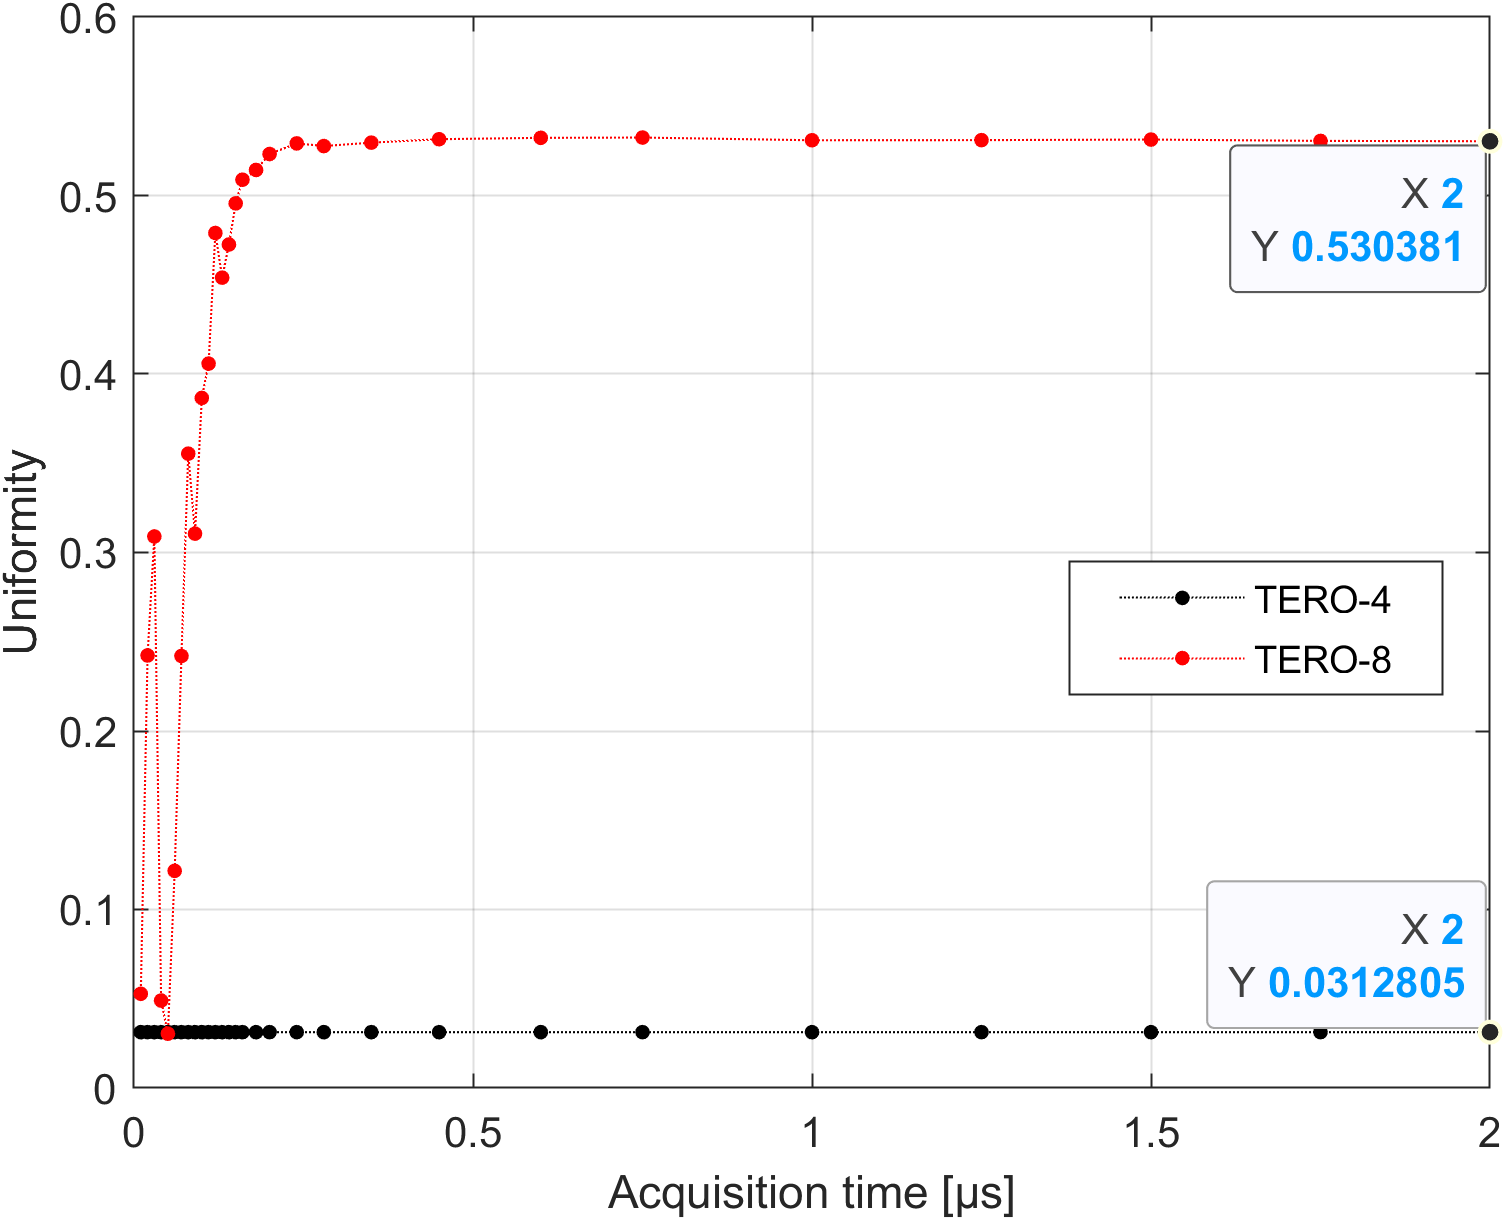
\includegraphics[width=0.8\linewidth]{images/all_intra_uniformity.png}
    \caption{\acrshort{puf} intra-uniformity}
    \label{fig:all_intra_uniformity}
\end{figure}

It was expected from the previous test about cell oscillations that the uniformity of the TERO-4 would be poor, due to the high number of equalities. From the 96.8\% of equality found, we know that 96.8\% of the generated bits are '0'. If we assume that the remaining 3.2\% of the bit are perfectly uniform, this would induce that $96.8\% + 3.2\%\times50\% = 98.4\%$ of the bits are '0', which corresponds to a uniformity of 1.6\%. The 3\% found is higher than this prediction, indicating that there is more '1' on the remaining bits than expected. Nevertheless, this proves that the TERO-4 uniformity is extremely low, at least for this specific device.\\


For the TERO-8, the oscillation of the uniformity at the beginning of the figure~\ref{fig:all_intra_uniformity} is also expected from the oscillation of the equalities at the same acquisition time. Once it is stabilised, the uniformity exceeds 50\% by 3\%, indicating that there is slightly more '1' than '0' in the bits response.\\

In both case, there is more '1' than expected, which could be either due to this specific device or to the implementation. This will be determined by the inter-device characterisation (~\ref{sec:inter_device_perf}).

\subsection{Reliability}


The \acrfull{relia} is the measure of the stability of each bit over multiple samples and is ideally equal to 100\%. This metric is shown in figure~\ref{fig:all_intra_reliability}. The TERO-4 reliability is constantly at 100\% while the TERO-8 reliability oscillates initially between 99 and 93\%, then stabilises at 97.7\% after $0.4\mu s$.

\begin{figure}[H]
    \centering
    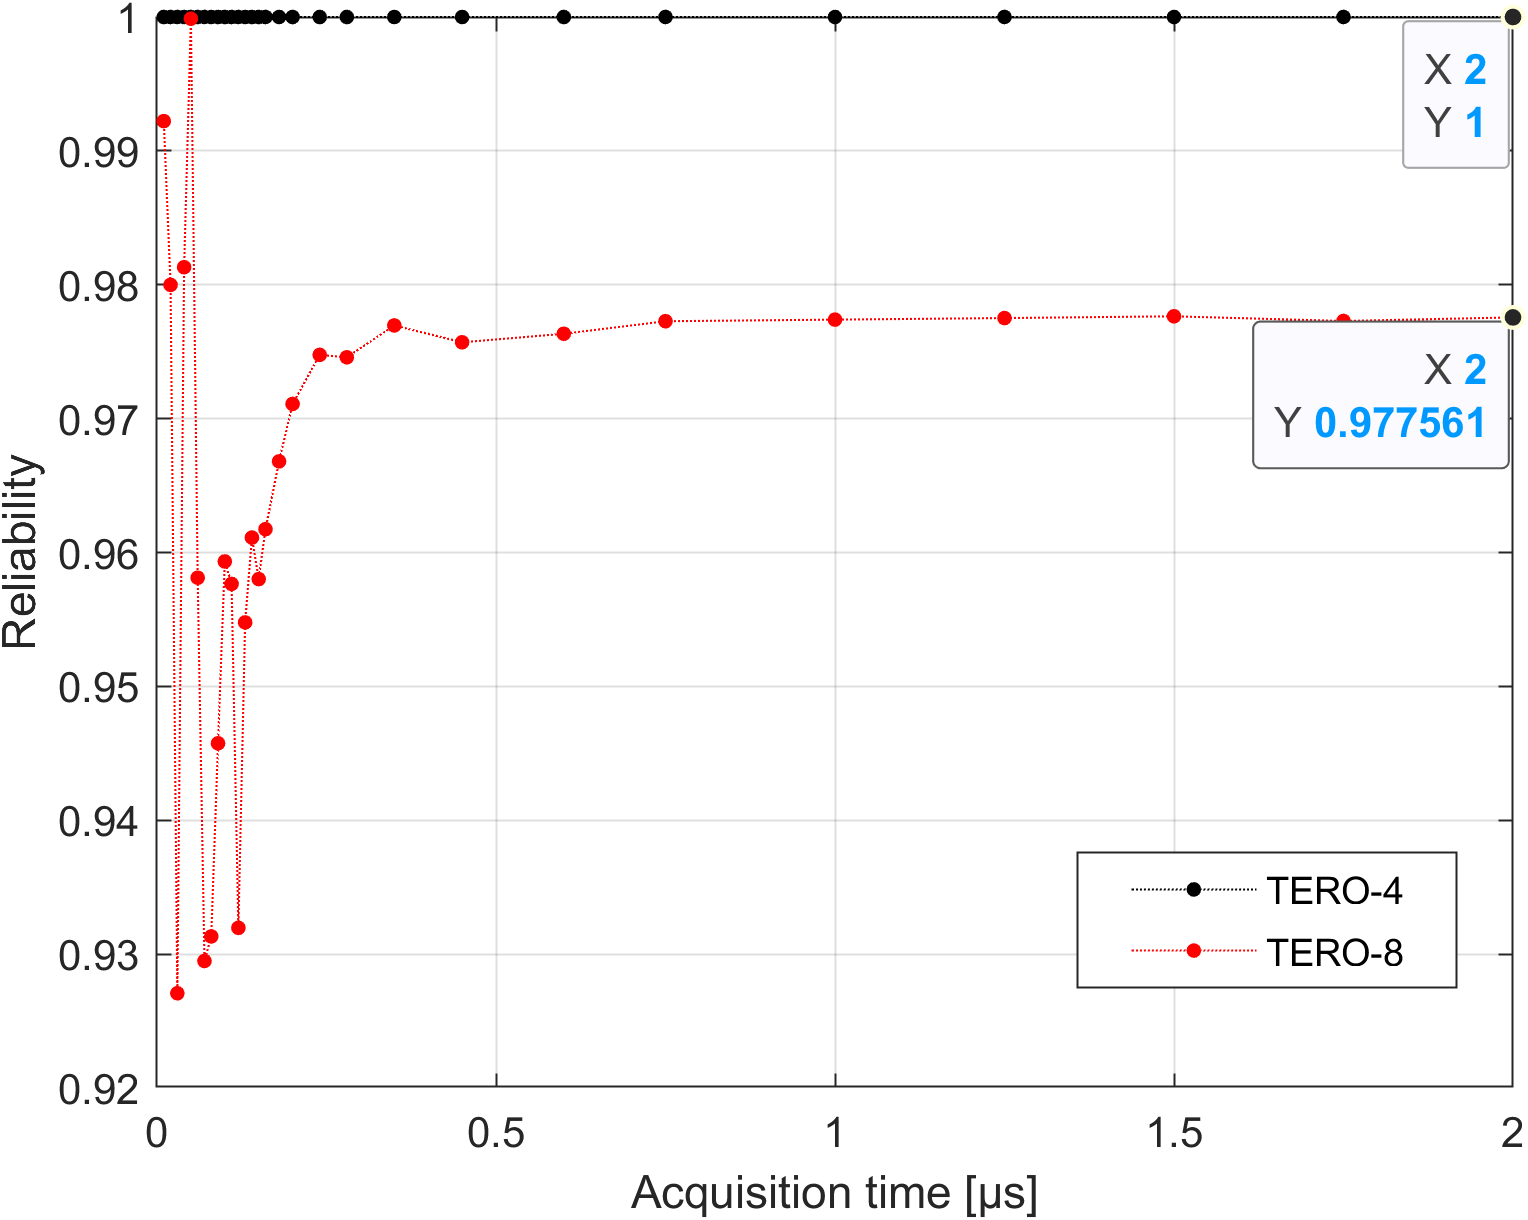
\includegraphics[width=0.8\linewidth]{images/all_intra_reliability.png}
    \caption{PUF intra-reliability}
    \label{fig:all_intra_reliability}
\end{figure}

The TERO-4 constant reliability is coherent with the fact that 63 of the 64 stabilise immediately, and therefore the response does not change anymore with the acquisition time. The fact that it is at 100\% reveals that the cell's final states are completely stable for this device over the 10 000 samples captured.\\

Once the TERO-8 cells have stabilised, the reliability found is comparable to the state of the art, but additional error correction techniques could increase the stability depending on the target application.\\

When we look at both the uniformity and reliability of the implementations, we can confirm that the TERO-4 does not provide good enough performance on this specific device while TERO-8 seems to produce correct performance. This also shows that an acquisition time higher than $0.5 \mu s$ does not provide any benefit to the results from this device. We choose $1 \mu s$ for the acquisition time used in the final tests, by assuming that the variation of this result between the devices is smaller than $0.5 \mu s$.


\section{Inter-device performances}

\label{sec:inter_device_perf}

The previous performance estimations are done on a single board and it is important to study the variation of those performances over multiple devices. The responses produced by different devices should be very unique and we can also check a systematic bias in the implementation for specific bits. In this test, the two TERO PUFs are uploaded on 33 BASYS-3 boards and the responses are recorded for an acquisition time of $1\mu s$. The device used in the previous test is at index 1.

\subsection{Inter-device uniformity}


\begin{figure}[H]
    \centering 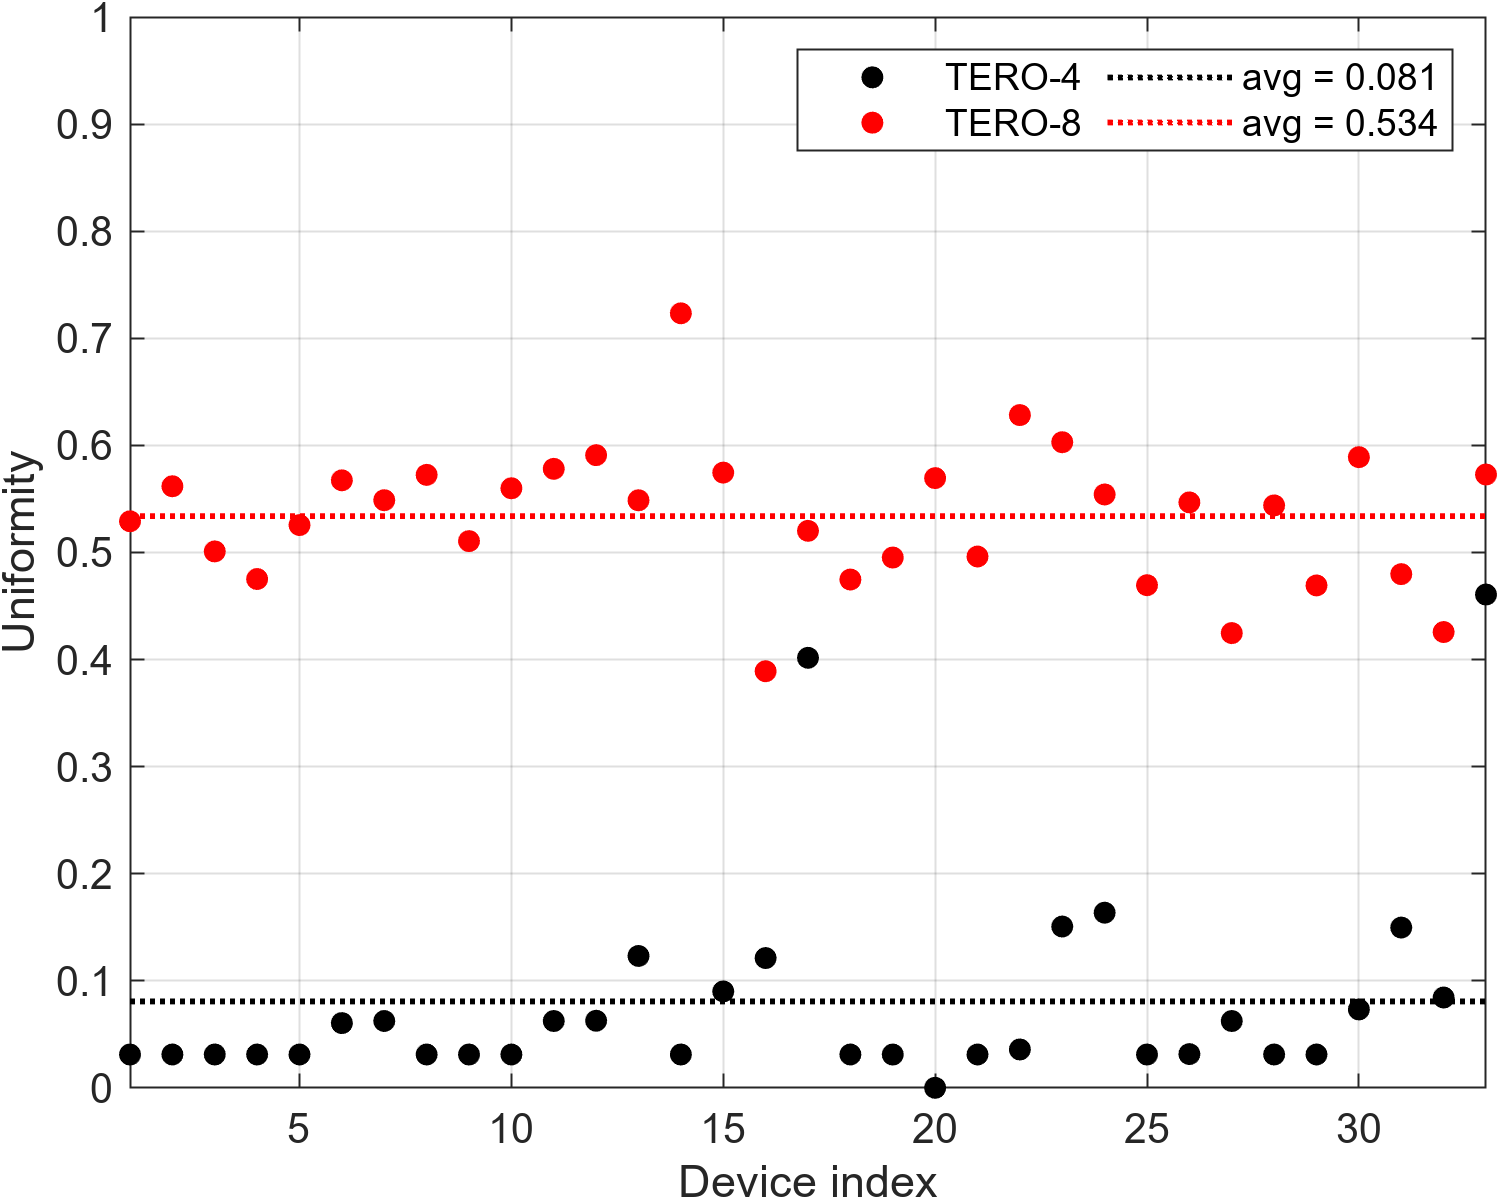
\includegraphics[width=0.8\linewidth]{images/tero_inter_uniformities.png}
    \caption{Inter-device uniformity's}
    \label{fig:tero_inter_uniformities}
\end{figure}


The TERO-4 uniformities of the 33 boards are represented in the figure~\ref{fig:tero_inter_uniformities}, with the dotted line for the average. 2 devices produce a uniformity higher than 40\%, while most of them stay below 8.0\% average. This proves that the poor uniformity found in the previous test (device at index 1) is not due to bad luck in the choice of the device but rather comes from the TERO-4 cells implementation itself.\\


The TERO-8 uniformities in figure~\ref{fig:tero_inter_uniformities} reveal that the device's uniformity from the previous test (53.0\%) was really representative of the 53.4\% average uniformity for this implementation. However, this also shows that this metric variation of this metrics between 39\% and 72\% depending on the device used.



\subsection{Inter-device reliability}
\label{subsec:inter_device_relia}

\begin{figure}[H]
    \centering 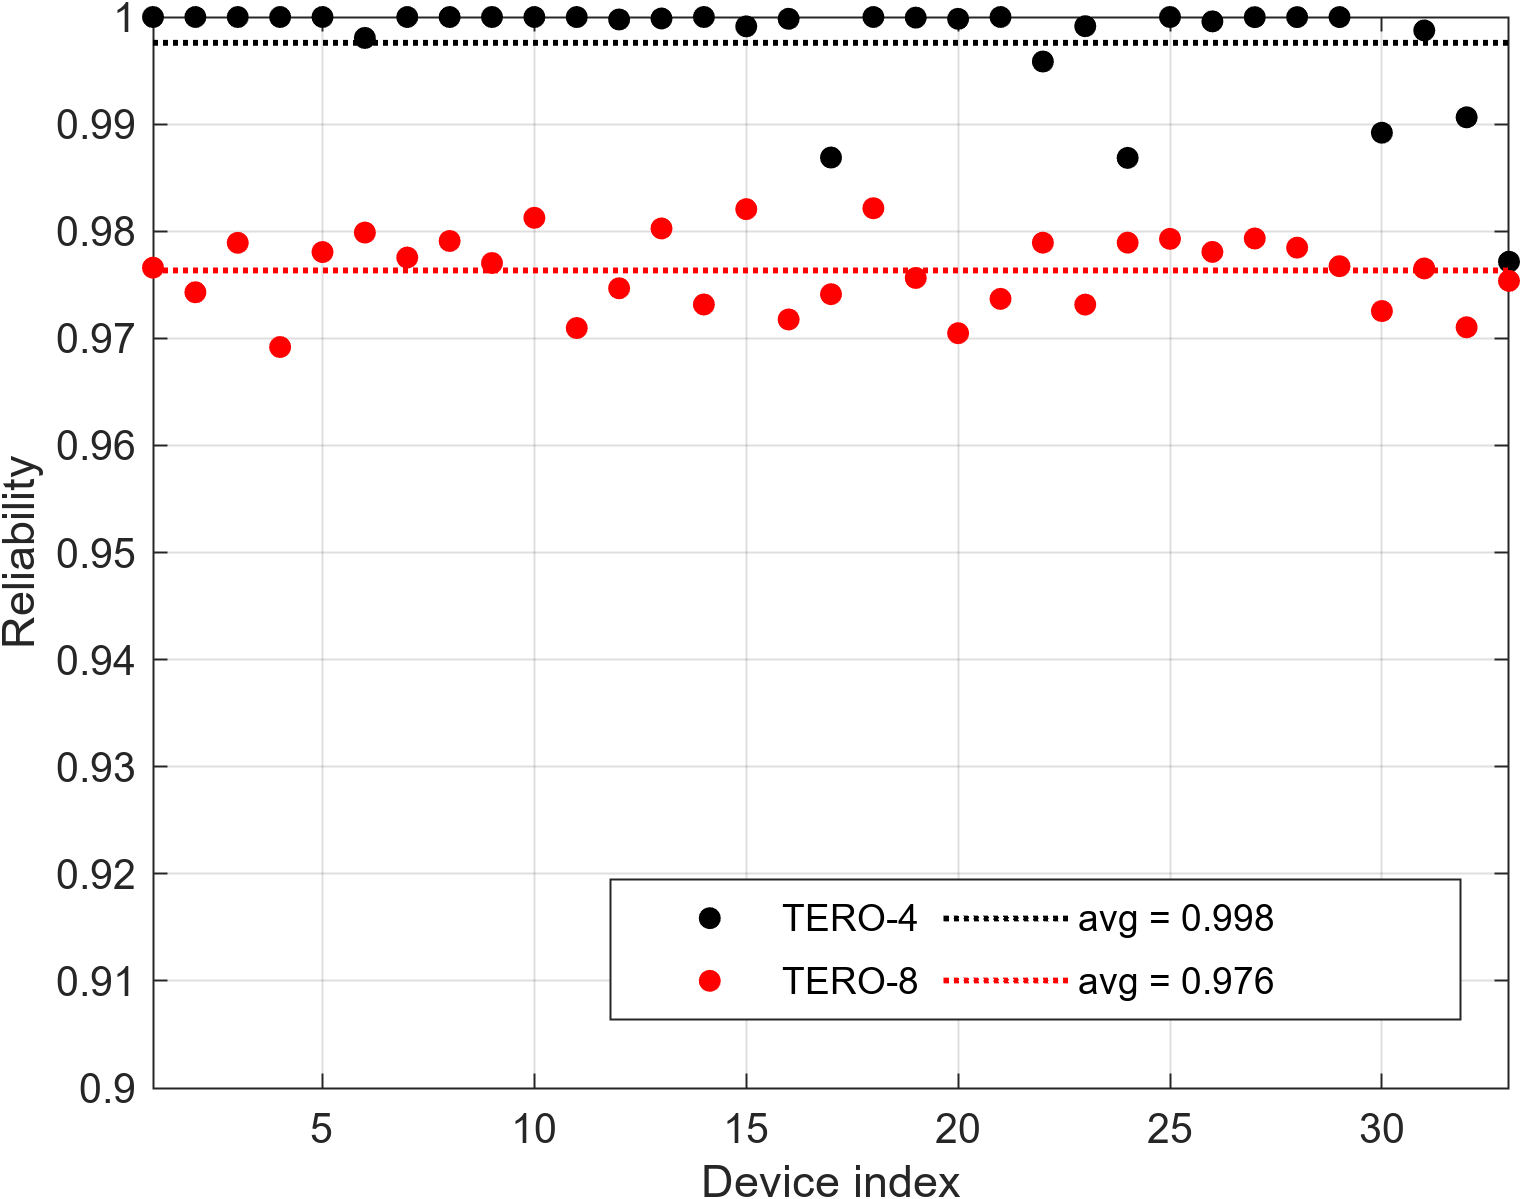
\includegraphics[width=0.8\linewidth]{images/tero_inter_reliabilities.png}
    \caption{Inter-device reliability's}
    \label{fig:tero_inter_reliabilities}
\end{figure}

Figure~\ref{fig:tero_inter_reliabilities} represent the TERO-4 reliability's. This indicates that most devices produce near-perfect reliability (99.8\% average). This also reveals that the device used in the previous test (index 1) was one of the devices that have perfect reliability over the 10 000 samples, but that is not always the case and a few devices produced a reliability below 99\%.\\


The TERO-8, displayed in figure~\ref{fig:tero_inter_reliabilities}, confirms that the value found on the previous test (97.7\%) was a good representation of the average (97.6\%) for the 33 devices. Furthermore, we can see that all the values are within a variation of 1\%.


\subsection{Bit-Aliasing}

Bit-aliasing is the measure of how likely is a specific bit to be '1' over all the devices. Ideally, this would be equal to 50\% for all the bits. However, since we only tested 33 devices, instead of looking only at the average, we should compare the distribution of the bit-aliasing values to the ideal distribution i.e. a binomial distribution of probability 50\% over 33 experiments (represented in green in figure~\ref{fig:tero_inter_aliasing}).

\begin{figure}[H]
    \centering 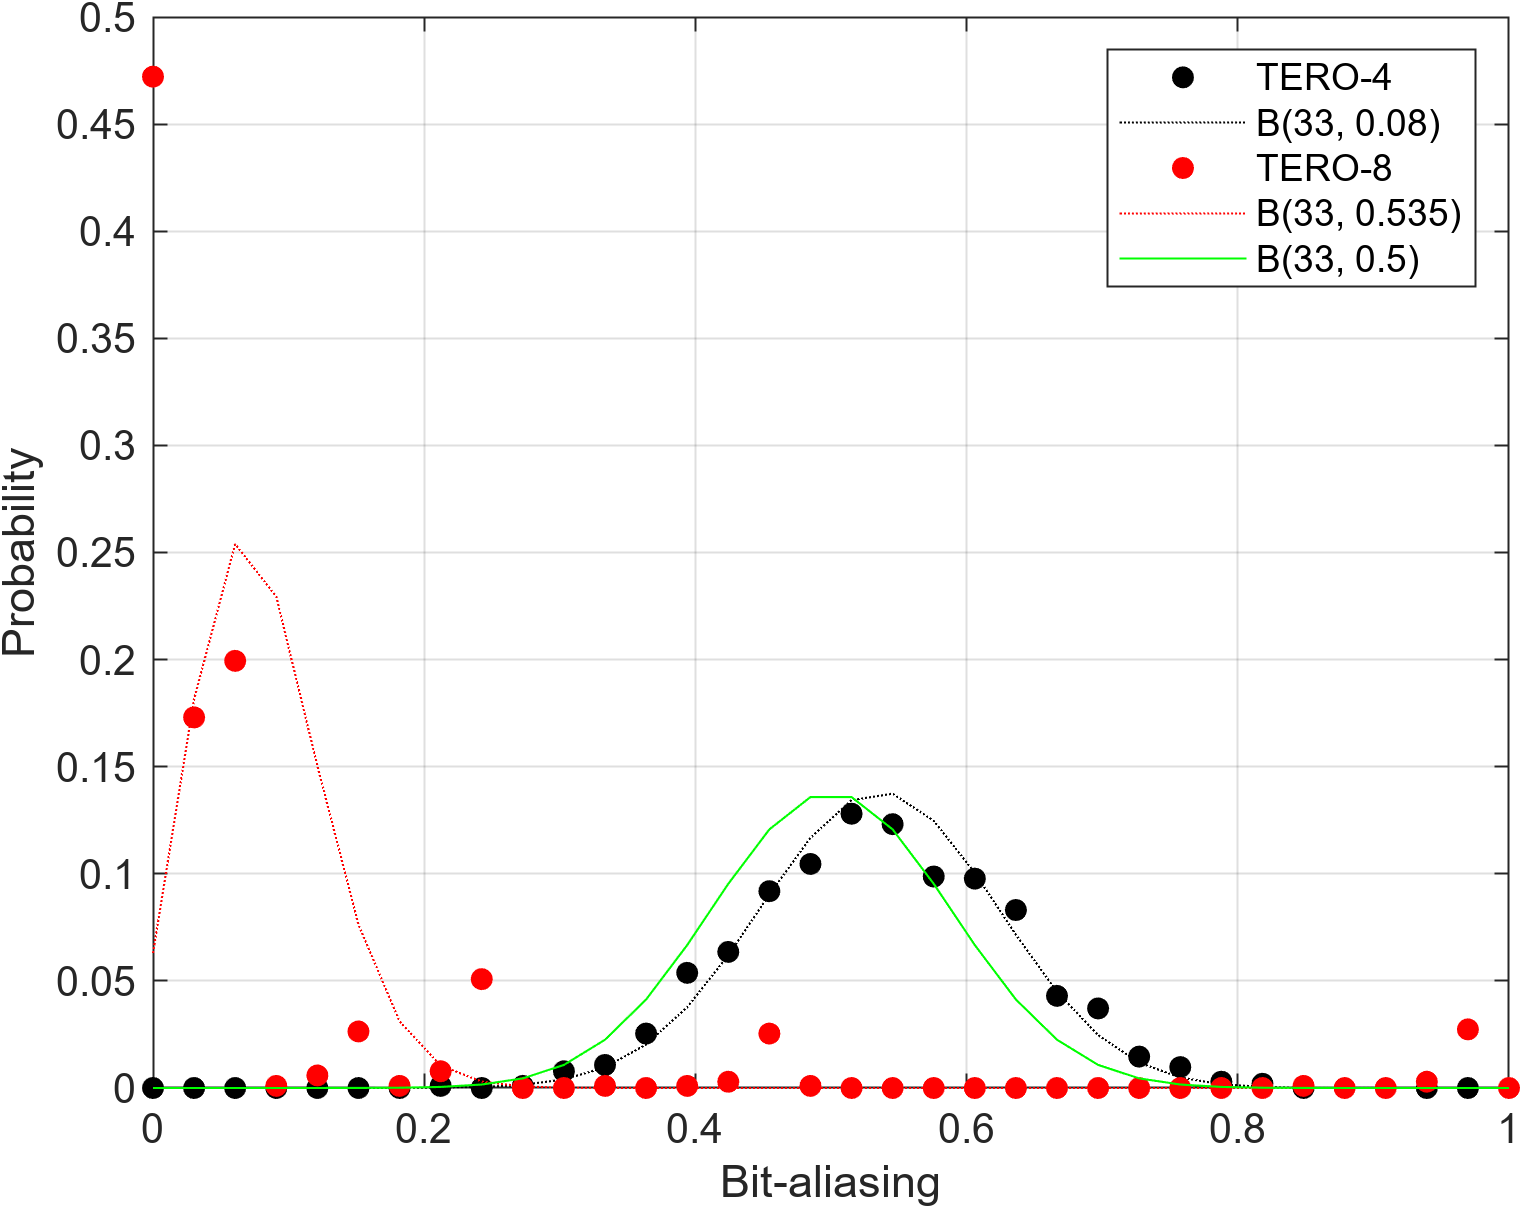
\includegraphics[width=0.8\linewidth]{images/tero_inter_aliasing.png}
    \caption{Inter-device bit-aliasing}
    \label{fig:tero_inter_aliasing}
\end{figure}

We already know that only 8.0\% of the TERO-4 bits are '1' for the average uniformity. Figure~\ref{fig:tero_inter_aliasing} reveals that almost 50\% of the bits are completely biased toward 0, meaning that they are always '0' in all the 33 devices tested. The average bit-aliasing is 8.0\% but the TERO-4 distribution does not follow a binomial distribution for this probability either. From the previous test, we know that the large number of bits equal to '0' in the device at index 1 is due to the large number of cells that do not oscillate. If we suppose that this is also the case in the other device, then this would mean that at least part of the cell that does not oscillate seems to always be the same regardless of the device. This indicates a bias in the implementation itself for specific cells.\\



The TERO-8 bit-aliasing distribution (figure~\ref{fig:tero_inter_aliasing}) follows closely a binomial distribution centred around its average of 53.5\%. This indicates that all the bits seem to give different response depending on the device, with a small overall bias of 3.5\% toward '1' which correspond almost to the 3.4\% excess of uniformity. This means that no bit is systematically at the same value but that there seems to be a global tendency for the cells in one array to produce a higher number of oscillations than the cells in the other array.



\subsection{Uniqueness}

The uniqueness is the measure of how different the responses of the different devices are in terms of hamming distance, with an ideal value of 50\%. The results for this metric are on the table~\ref{tab:uniqueness}.

%Q?
%Decimal ? or %
\begin{table}[H]
    \centering
    \begin{tabular}{|c|c|}
        \hline
            & Uniqueness\\
         \hline
         TERO-4 & 8.2\%\\
         \hline
         TERO-8 & 49.4\%\\
         \hline
    \end{tabular}
    \caption{Uniqueness}
    \label{tab:uniqueness}
\end{table}

The TERO-4 responses only produce an 8.2\% of uniqueness, which is understandable since we know from the bit-aliasing that a large part of the bits response is always '0'. For the TERO-8 however, the responses have a uniqueness of 49.42\% over the 33 devices tested, which is close to the ideal value. 


\begin{table}[H]
    \centering
    \begin{tabular}{|c|c|c|c|c|}
        \hline
            & Uniformity & Reliability & Bit-aliasing & Uniqueness\\
         \hline
         TERO-4 & 8.1\% & 99.8\% & 8.0\% & 8.2\%\\
         \hline
         TERO-8 & 53.4\% & 97.6\% & 53.5\% & 49.4\%\\
         \hline
    \end{tabular}
    \caption{Inter-device performances}
    \label{tab:summary_inter}
\end{table}

It appears clearly that the TERO-4 implementation does not provide the desired performances in terms of uniformity, bit-aliasing and uniqueness. This is most likely due to the cells that systematically stabilise without any oscillation. We therefore consider this implementation to not be usable and it will not be discussed in the rest of this chapter.

\newpage
\section{Error correction}


The TERO-8 average reliability is 97.63\%, which, depending on the target application, may not be good enough. We will therefore evaluate the improvement brought by the ECC described in \ref{subsec:demon_feature_bch}.\\

The responses of the ECC implementation are recorded for the same acquisition time ($1\mu s$) over the 33 BASYS-3 boards in the same condition as the previous test. The table ~\ref{tab:raw_&_ecc_perf} contains all the inter-device metrics of the initial TERO-8 implementation ("Full"), the reduced version of it with only 171 bits ("Reduced") and the response of the BCH decoder for error correction ("ECC").

\begin{table}[H]  
  \centering
    \begin{tabular}{|c|c|c|c|c|c|}
        \hline
        \textbf{TERO-8} &  Response's size & RE & UF & UQ & BA\\
        \hline
        Full & 1023 bits & 97.6\% & 53.4\% & 49.4\% & 53.5\%\\
        \hline
        Reduced & 171 bits & 97.7\% & 53.4\% & 49.9\% & 54.4\%\\
        \hline
        ECC & 171 bits & 99.9\% & 53.5\% & 49.9\% & 54.4\%\\
        \hline
    \end{tabular}
   \caption{\label{tab:raw_&_ecc_perf}TERO-8 performances without and with ECC}
\end{table}

First, we can observe that the performances of the reduced version (without ECC) are very similar to the full one. Therefore, any improvement due to the ECC on the reduced response can be supposed to be equally effective on an entire response.

Moreover, when we compare the reliability between the reduced response and the ECC one, it goes from 97.71\% to 99.90\%, which is an improvement. At the same time, the other performances remain substantially the same.

As expected, using this technique, we significantly increase the performance of the TERO-8 without any downside other than the additional FPGA resources used (discussed in \ref{subsec:fpga_usage_area}). Depending on the target application, reliability higher than 99.9\% can still be required. In this case, a BCH supporting a higher number of errors should be used.\\

\newpage
\section{Comparison with existing implementations}

The performance produced by the TERO-8 implementation are comparable to both other \acrshort{teropuf} implementation (table~\ref{tab:tero_impls}) and other \acrshort{puf} techniques using an Artix-7 for implementation (table~\ref{tab:artix7_impl}), with only the \acrshort{ecc} version giving a reliability in line with the literature. 

\begin{table}[H]
    \centering
    \begin{tabular}{|c|c|c|c|c|c|c|c|}
         \hline
         \textbf{method} & \textbf{\acrshort{relia}} & \textbf{\acrshort{unif}} & \textbf{\acrshort{uniq}} & \textbf{\acrshort{bit-alia}} & \textbf{device} & \textbf{Ref}\\
         \hline\hline
         TERO & 98.3\% & - & 48\% & - & Cyclone-II & \cite{bossuet_puf_2014}\\
         \hline\hline
         TERO & 99.99\% & - & 46.7\% & - & Altera DE2 & \cite{bossuet_puf_2014}\\
         \hline
         TERO & 97.4\% & - & 48.5\% & - & Spartan-6 & \cite{marchand_implementation_2017}\\
          & 98.2\% & - & 47.6\% & - & Cyclone-V & \\
         \hline
         PDL-TERO & 98.8\% & - & 49.32\% & - & Spartan-3 & \cite{ardakani_improving_2018}\\
         \hline\hline
         \textbf{RAW (full)} & \textbf{97.6\%} & \textbf{53.4\%} & \textbf{49.4\%} & \textbf{53.5\%} & \textbf{Artix-7} & \textbf{This}\\ 
         \textbf{ECC} & \textbf{99.9\%} & \textbf{53.5\%} & \textbf{49.9\%} & \textbf{54.4\%} & & \textbf{work}\\
         \hline
    \end{tabular}
    \caption{\acrshort{teropuf} implementations on FPGA}
    \label{tab:tero_impls}
\end{table}



\begin{table}[H]
    \centering
    \begin{tabular}{|c|c|c|c|c|c|c|c|}
         \hline
         \textbf{method} & \textbf{\acrshort{relia}} & \textbf{\acrshort{unif}} & \textbf{\acrshort{uniq}} & \textbf{\acrshort{bit-alia}} & \textbf{Ref}\\
         \hline\hline
         APUF & 99.55\% & 51.84\% & 46.21\% & -  & \cite{anandakumar_implementation_2022}\\
         \hline
         XOR-APUF & 99.41\% & 50.73\% & 48.69\% &  - & \cite{anandakumar_implementation_2022}\\
         \hline
         BST-APUF & 99.99\% & - & 49.1\% & 50.3\% & \cite{he_highly_2020}\\
         \hline
         ROPUF & 99.19\% & 51.01 & 47.86\% & 51.01\% & \cite{de_weerdt_implementation_2021}\\
         \hline
         BST-ROPUF & 99.99\% & 46.78\% & 48.64\% & - & \cite{he_highly_2021}\\
         \hline
         RWC-SRAMPUF & 98.92\% & 55.38\% & 37.36\% & 46.89\% & \cite{cicek_new_2022}\\
         \hline
         Flip-Flop PUF & ~99\% & 49.2\% & - & 48.96\% & \cite{khan_symmetric_2020}\\
         \hline\hline
         \textbf{RAW (full)} & \textbf{97.6\%} & \textbf{53.4\%} & \textbf{49.4\%} & \textbf{53.5\%} & \textbf{This}\\ 
         \textbf{ECC} & \textbf{99.9\%} & \textbf{53.5\%} & \textbf{49.9\%} & \textbf{54.4\%} & \textbf{work}\\
         \hline
    \end{tabular}
    \caption{\acrshort{puf} implementations on Artix-7}
    \label{tab:artix7_impl}
\end{table}

\newpage
\section{Demonstration}

Using the python module (appendix~\ref{appendix:python_mod}) and a USB cable for \acrshort{uart} communication between the \acrshort{fpga} and a computer, we can demonstrate the different responses of the implementation: the raw response (figure~\ref{fig:demo_raw}), the response after \acrshort{ecc} (figure~\ref{fig:demo_ecc}) and the \acrshort{sha} key generated (figure~\ref{fig:demo_sha}).

\begin{figure}[H]
    \centering
    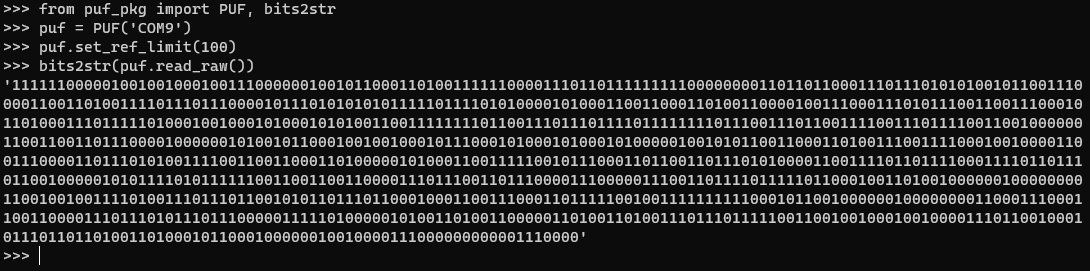
\includegraphics[width=\linewidth]{images/demo_raw.png}
    \caption{Demonstration raw response}
    \label{fig:demo_raw}
\end{figure}

\begin{figure}[H]
    \centering
    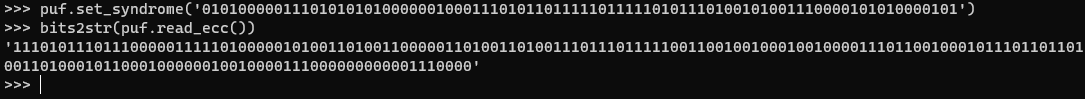
\includegraphics[width=\linewidth]{images/demo_ecc.png}
    \caption{Demonstration ECC response}
    \label{fig:demo_ecc}
\end{figure}

\begin{figure}[H]
    \centering
    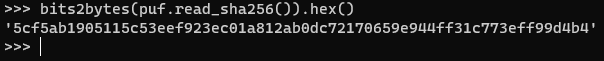
\includegraphics[width=\linewidth]{images/demo_sha.png}
    \caption{Demonstration SHA-256 key}
    \label{fig:demo_sha}
\end{figure}


